

\begin{frame}{Overview}

 \begin{block}{Hardware}
  \begin{itemize}
   \item Graphics Processing Units
   \item Many Integrated Cores (Xeon Phi family)
  \end{itemize}
 \end{block}

 \begin{block}{Software}
  \begin{itemize}
   \item CUDA
   \item OpenCL
   \item Parallel Primitives
  \end{itemize}
 \end{block}

 \begin{block}{Performance Modeling}
  \begin{itemize}
   \item Identifying Bottlenecks
   \item Modeling by Example
  \end{itemize}
 \end{block}


\end{frame}


%%
%% Part C: Hardware
%%

%% 6. GPUs


% \begin{frame}[fragile]
% \frametitle{GPU Overview}
%  \begin{block}{Computing Architecture Schematic}
%   \begin{center}
%    \includegraphics[width=0.8\textwidth]{figures/cpu-gpu-coarse.pdf}
%   \end{center}
% 
%  
%  \begin{itemize}
%   \item \vspace*{1.03cm}
%  \end{itemize}
%  \end{block}
% 
% \end{frame}

\begin{frame}[fragile]
\frametitle{GPU Overview}
 \begin{block}{Computing Architecture Schematic}
  \begin{center}
   \includegraphics[width=0.8\textwidth]{figures/cpu-gpu-detail.pdf}
  \end{center}

 \begin{itemize}
  \item Good for large FLOP-intensive tasks, high memory bandwidth
  \item PCI-Express can be a bottleneck
  \item $\gg 10$-fold speedups (usually) not backed by hardware
 \end{itemize}
 \end{block}

\end{frame}

\begin{frame}{GPU Overview}
 \begin{center} \includegraphics[width=0.95\textwidth]{figures/gpu-schematic} \end{center}
 
 \begin{block}{Details}
  \begin{itemize}
   \item Workgroups consist of 32-64 hardware threads
   \item Up to 24 hardware workgroups
   \item Shared memory small: approx. 32-64 KB
  \end{itemize}

 \end{block}

\end{frame}


% Explain SIMT
\begin{frame}{GPU Overview}
 \begin{block}{Reminder: AVX}
   \begin{itemize}
    \item One instruction for all elements of a vector register
   \end{itemize}
 \end{block}

 \begin{center} \includegraphics[width=0.9\textwidth]{figures/avx} \end{center}

 %\pause 
 \begin{block}{Single Instruction Multiple Threads (SIMT)}
  \begin{itemize}
   \item One instruction for all threads in workgroup
   \item Each thread has separate registers
   \item Efficient if all threads execute the same instruction
  \end{itemize}
 \end{block}

 \begin{center} \includegraphics[width=0.9\textwidth]{figures/simt} \end{center}

\end{frame}


% GDDRAM


\begin{frame}{GPU Overview}

 \begin{block}{GDDR5}
   \begin{itemize}
    \item Optimized for throughput
    \item Channel width: multiple of 32 bits
    \item High bus width: 256 bits, 384 bits
   \end{itemize}
 \end{block}

 %\pause
 
 \begin{block}{Structured Memory Access}
   \begin{itemize}
    \item Memory controllers use 32/64/128 byte transactions
    \item Partial transactions degrade effective bandwidth
   \end{itemize}
 \end{block}

 %\pause
%   \only<1-3>{\begin{center} \includegraphics[width=0.9\textwidth]{figures/memory-access-good} \end{center}}
%   \only<4>{\begin{center} \includegraphics[width=0.9\textwidth]{figures/memory-access-okay} \end{center}}
%   \only<5>{\begin{center} \includegraphics[width=0.9\textwidth]{figures/memory-access-bad} \end{center}}
 \begin{center} \includegraphics[width=0.9\textwidth]{figures/memory-access-bad} \end{center}

\end{frame}




% Interconnect: Plot PCI-Express bandwidth


\begin{frame}{GPU Overview}

 \begin{block}{Host-Device Communication}
  \begin{itemize}
   \item PCI-Express v2: $\hphantom{1}$8 GB/sec max
   \item PCI-Express v3: 16 GB/sec max
   \item Latency: about 10 $\mu$s
  \end{itemize}

 \end{block}


 \begin{center}
  \includegraphics[width=0.48\textwidth]{figures/pcie-time-5-crop} \hfill
  \includegraphics[width=0.48\textwidth]{figures/pcie-bandwidth-5-crop}
 \end{center}
\end{frame}



%% 7. MICs

% Explain KNC
\begin{frame}{Many Integrated Core Architecture}
 
 \begin{block}{Background}
  \begin{itemize}
   \item Many-core architecture by Intel
   \item ``Just recompile'' existing OpenMP-enabled code
   \item Current: Knights Corner (Q4 2012)
   \item Upcoming: Knights Landing (Q1 2016)
  \end{itemize}
 \end{block}
 
 \begin{center}
  \includegraphics[width=0.5\textwidth]{figures/xeon-phi}
 \end{center}

\end{frame}

\begin{frame}{Many Integrated Core Architecture}
 
 \begin{block}{Knight Corner: Technical Details}
  \begin{itemize}
   \item High memory bandwidth: 320 GB/sec ideal, 160 GB/sec real
   \item High compute power: 1 TFLOP/sec (fp64)
   \item Fixed main memory: 8 or 16 GB
   \item Custom operating system on board
  \end{itemize}
 \end{block}
 
 \vspace*{-0.5cm}
 \begin{center}
  \includegraphics[width=0.7\textwidth]{figures/stream}
 \end{center}

\end{frame}


\begin{frame}{Many Integrated Core Architecture}
 
 \begin{block}{Knights Corner: Problems}
  \begin{itemize}
   \item Very low single-thread performance
   \item ``Just recompile'' almost never enough
   \item PCI-Express communication slower than for GPUs
   \item Even Intel now recommends Haswell-Xeons over Knights Corner
  \end{itemize}
 \end{block}
 
 %\pause
 \begin{center}
  \includegraphics[width=0.65\textwidth]{figures/xkcd-someone-wrong} \\
  {\scriptsize http://xkcd.com/386/}
 \end{center}

\end{frame}


% Explain new stuff for KNL

\begin{frame}{Many Integrated Core Architecture}
 
 \begin{block}{KNL: Compute}
  \begin{itemize}
   \item 72 cores
   \item Energy-efficient IA cores
   \item 3x single-thread performance vs. KNC
   \item Binary compatibility with Xeon line
   \item 3+ TFLOPS in double precision
  \end{itemize}
 \end{block}

 \begin{block}{KNL: On-Package Memory}
  \begin{itemize}
   \item 16 GB
   \item 5x bandwidth vs. DDR4
   \item 5x power efficiency vs. DDR4
  \end{itemize}
 \end{block}
 
\end{frame}


\begin{frame}{Many Integrated Core Architecture}
 
 \begin{block}{KNL Schematic}
  \begin{itemize}
   \item 36 tiles interconnected by 2D mesh
   \item Each tile: 2 cores, 2 vector units per core, 1 MB L2 cache
  \end{itemize}
 \end{block}
 
 \begin{center}
  \includegraphics[width=0.5\textwidth]{figures/knl-schematic} \\
 \end{center}
\end{frame}

\begin{frame}{Many Integrated Core Architecture}
 
 \begin{block}{HBM: Cache Mode}
  \begin{itemize}
   \item No code changes necessary
   \item Cache misses expensive
  \end{itemize}
 \end{block}

 \begin{block}{HBM: Flat Mode}
  \begin{itemize}
   \item MCDRAM mapped to physical address space
   \item Exposed as NUMA node
   \item Accessed through memkind library or numactl
  \end{itemize}
 \end{block}

 \begin{block}{HBM: Hybrid Mode}
  \begin{itemize}
   \item Combination of the above two
   \item Get the best and worst of two worlds
  \end{itemize}
 \end{block}

\end{frame}




%%
%% Part D: Software
%%

\begin{frame}{Overview} \begin{center} \Large Software: CUDA \end{center} \end{frame}


%% 8. CUDA

\begin{frame}[fragile]{CUDA}
 
 \begin{block}{About}
  \begin{itemize}
   \item Initial release in 2007
   \item Proprietary programming model by NVIDIA
   \item C++ with extensions
   \item Proprietary compiler extracts GPU kernels
  \end{itemize}
 \end{block}

 \begin{block}{Software Ecosystem}
  \begin{itemize}
   \item Vendor-tuned libraries: cuBLAS, cuSparse, cuSolver, cuFFT, etc.
   \item Python bindings: pyCUDA
   \item Community projects: CUSP, MAGMA, ViennaCL, etc.
  \end{itemize}
 \end{block}

\end{frame}

% Slide series: From OpenMP to CUDA. Mention shitty OpenACC?

% \begin{frame}[fragile]{CUDA}
%  
%  \begin{block}{Programming in CUDA}
%   \begin{lstlisting}
% void work(double *x, double *y, double *z, int N)
% {
% 
% 
%   for (size_t i=0; i<N; ++i)
%     z[i] = x[i] + y[i];
% }
%   \end{lstlisting}
%   \begin{lstlisting}
% int main(int argc, char **argv)
% {
%   int N = atoi(argv[1]);
%   double *x = malloc(N*sizeof(double));
%   ...
%   
%   ...
%   work(x, y, z, N); // call kernel
%   ...
%  
%  
%   free(x);
% }  
%   \end{lstlisting}
%  \end{block}
% \end{frame}
% 
% %%%%%%%%%%%%%%%%%%%%5
% 
% \begin{frame}[fragile]{CUDA}
%  
%  \begin{block}{Programming in CUDA}
%   \begin{lstlisting}
% void work(double *x, double *y, double *z, int N)
% {
% 
%   #pragma omp parallel for
%   for (size_t i=0; i<N; ++i)
%     z[i] = x[i] + y[i];
% }
%   \end{lstlisting}
%   \begin{lstlisting}
% int main(int argc, char **argv)
% {
%   int N = atoi(argv[1]);
%   double *x = malloc(N*sizeof(double));
%   ...
%   
%   ...
%   work(x, y, z, N); // call kernel
%   ...
%  
%  
%   free(x);
% }  
%   \end{lstlisting}
%  \end{block}
% \end{frame}
% 
% %%%%%%%%%%%%%%%%%%%%5
% 

\begin{frame}[fragile]{CUDA}
 
 \begin{block}{Programming in CUDA}
  \begin{lstlisting}
void work(double *x, double *y, double *z, int N)
{
  #pragma omp parallel
{ int thread_id = omp_get_thread_num();
  for (size_t i=thread_id; i<N; i += omp_get_num_threads())
    z[i] = x[i] + y[i];
} }
  \end{lstlisting}
  \begin{lstlisting}
int main(int argc, char **argv)
{
  int N = atoi(argv[1]);
  double *x = malloc(N*sizeof(double));
  ...
  
  ...
  work(x, y, z, N); // call kernel
  ...
 
 
  free(x);
}  
  \end{lstlisting}
 \end{block}
\end{frame}


%%%%%%%%%%%%%%%%%%%%5


\begin{frame}[fragile]{CUDA}
 
 \begin{block}{Programming in CUDA}
  \begin{lstlisting}
__global__ void work(double *x, double *y, double *z, int N)
{

  int thread_id = blockIdx.x*blockDim.x + threadIdx.x;
  for (size_t i=thread_id; i<N; i += blockDim.x * gridDim.x)
    z[i] = x[i] + y[i];
}
  \end{lstlisting}
  \begin{lstlisting}
int main(int argc, char **argv)
{
  int N = atoi(argv[1]);
  double *x = malloc(N*sizeof(double));
  cudaMalloc(&gpu_x, N*sizeof(double));
  cudaMemcpy(gpu_x, x, N*8, cudaMemcpyHostToDevice);
  ...
  work<<<128, 256>>>(x, y, z, N); // call kernel
  ...
  cudaMemcpy(gpu_x, x, N*8, cudaMemcpyDeviceToHost);
  ...
  free(x);
}  
  \end{lstlisting}
 \end{block}
\end{frame}

%%%%%%%%%%%%%%%%%%%%5

\begin{frame}[fragile]{CUDA}

 \begin{center}
%  \only<1>{ \vspace*{1.04cm} \includegraphics[width=\textwidth]{copy-kernel-gpu-1}}
%  \only<2>{                  \includegraphics[width=\textwidth]{copy-kernel-gpu-full}}
  \includegraphics[width=\textwidth]{copy-kernel-gpu-full}
 \end{center}


\end{frame}

%%%%%%%%%%%%%%%%%%%%5

\begin{frame}[fragile]{CUDA}

\begin{block}{Thread Control (1D)}
 \begin{itemize}
  \item Local ID in block: \lstinline|threadIdx.x|
  \item Threads per block: \lstinline|blockDim.x|
  \item ID of block: \lstinline|blockIdx.x|
  \item No. of blocks: \lstinline|gridDim.x|
 \end{itemize}
\end{block}

\begin{block}{Recommended Default Values}
 \begin{itemize}
  \item Typical block size: 256 or 512
  \item Typical number of blocks: 256
  \item At least $10\,000$ logical threads recommended
 \end{itemize}
\end{block}

\end{frame}

%%%%%%%%%%%%%%%%%%%%5


% Revisit strided and offset memory access

\begin{frame}[fragile]{CUDA Example}

\begin{block}{Offset Memory Access}
  \begin{lstlisting}
__global__ 
void work(double *x, double *y, double *z, int N, int k)
{
  int thread_id = blockIdx.x*blockDim.x + threadIdx.x;
  for (size_t i=thread_id; i<N; i += blockDim.x * gridDim.x)
    z[i+k] = x[i+k] + y[i+k];
}  
  \end{lstlisting}
\end{block}

\vspace*{-0.5cm}
\begin{center}
 \includegraphics[width=0.6\textwidth]{figures/offset}
\end{center}

\end{frame}




\begin{frame}[fragile]{CUDA Example}

\begin{block}{Strided Memory Access}
  \begin{lstlisting}
__global__ 
void work(double *x, double *y, double *z, int N, int k)
{
  int thread_id = blockIdx.x*blockDim.x + threadIdx.x;
  for (size_t i=thread_id; i<N; i += blockDim.x * gridDim.x)
    z[i*k] = x[i*k] + y[i*k];
}  
  \end{lstlisting}
\end{block}

\vspace*{-0.5cm}
\begin{center}
 \includegraphics[width=0.6\textwidth]{figures/stride}
\end{center}

\end{frame}


%%

\begin{frame}[fragile]{CUDA Example}

\begin{block}{Strided Memory Access}
  \begin{itemize}
   \item Array of structs problematic
  \end{itemize}
  \begin{lstlisting}  
typedef struct particle
{
  double pos_x; double pos_y; double pos_z;
  double vel_x; double vel_y; double vel_z;
  double mass;
} Particle;
  
__global__ 
void increase_mass(Particle *particles, int N)
{
  int thread_id = blockIdx.x*blockDim.x + threadIdx.x;
  for (int i=thread_id; i<N; i += blockDim.x * gridDim.x)
    particles[i].mass *= 2.0;
}  
  \end{lstlisting}
\end{block}

\end{frame}

%%%

\begin{frame}[fragile]{CUDA Example}

\begin{block}{Strided Memory Access}
  \begin{itemize}
   \item Workaround: Structure of Arrays
  \end{itemize}
  \begin{lstlisting}  
typedef struct particles
{
  double *pos_x; double *pos_y; double *pos_z;
  double *vel_x; double *vel_y; double *vel_z;
  double *mass;
} Particle;
  
__global__ 
void increase_mass(Particle *particles, int N)
{
  int thread_id = blockIdx.x*blockDim.x + threadIdx.x;
  for (int i=thread_id; i<N; i += blockDim.x * gridDim.x)
    particles.mass[i] *= 2.0;
}  
  \end{lstlisting}
\end{block}

\end{frame}


\begin{frame}{Overview} \begin{center} \Large Software: OpenCL \end{center} \end{frame}



\begin{frame}{OpenCL Heterogeneity}

 \begin{block}{OpenCL Releases}
   \begin{itemize}
    \item OpenCL 2.2 (recently)
    \item OpenCL 2.1 (2015)
    \item OpenCL 2.0 (2013)
    \item OpenCL 1.2 (2011)
    \item OpenCL 1.1 (2010)
    \item OpenCL 1.0 (2009)
   \end{itemize}
 \end{block}

 %\pause
 \begin{block}{OpenCL Support in SDKs}
   \begin{itemize}
    \item 2.2: -
    \item 2.1: -
    \item 2.0: AMD, Intel (Win), Qualcomm
    \item 1.2: Apple, Beignet, Intel (Linux), Imagination, NVIDIA, pocl, Vivante
    \item 1.1: ARM, Sony, TI
    \item 1.0: Altera, Xilinx
   \end{itemize}
 \end{block}
 
\end{frame}



\begin{frame}{OpenCL Heterogeneity}

 \begin{block}{The Veto Problem}
   \begin{itemize}
    \item What if a major vendor stops OpenCL SDK development?
    \item What if SPIR-V is not broadly available?
   \end{itemize}
 \end{block}

 %\pause
 \begin{block}{Possible Reasons for Slow OpenCL SDK Development}
   \begin{itemize}
    \item Proprietary alternative available
    \item ``Will help competitor more than us''
    \item Development too expensive
   \end{itemize}
 \end{block}
 
\end{frame}
% 


\begin{frame}{OpenCL Heterogeneity}

 \begin{block}{How to Encourage?}
 \end{block}

 %\pause
 
 \begin{center}
  \includegraphics[width=0.2\textwidth]{figures/opencl} \ \ \ \ 
  \includegraphics[width=0.5\textwidth]{figures/vulkan-logo}\\[1.5em]
  Make OpenCL a prerequisite for Vulkan certification?
 \end{center}
 
\end{frame}

\begin{frame}{Overview} \begin{center} \Large Software: Parallel Primitives \end{center} \end{frame}
%% 10. Parallel Primitives

% Reductions

\begin{frame}{Parallel Primitives}

\begin{block}{Reductions}
  \begin{itemize}
   \item Use $N$ values to compute $1$ result value
   \item Examples: Dot-products, vector norms, etc.
  \end{itemize}
\end{block}

\begin{block}{Reductions with Few Threads}
  \begin{itemize}
   \item Decompose $N$ into chunks for each thread
   \item Compute chunks in parallel
   \item Merge results with single thread
  \end{itemize}
\end{block}

\begin{center} \includegraphics[width=0.7\textwidth]{figures/reductions-thread} \end{center}

\end{frame}





\begin{frame}{Parallel Primitives}

\begin{block}{Reductions with Many Threads}
  \begin{itemize}
   \item Decompose $N$ into chunks for each workgroup
   \item Use fast on-chip synchronization within each workgroup
   \item Sum result for each workgroup separately
  \end{itemize}
\end{block}

\begin{center} \includegraphics[width=0.8\textwidth]{figures/inner-product-kernel} \end{center}


\end{frame}




% \begin{frame}[fragile]{Parallel Primitives}
% 
%  \begin{block}{Reductions with Many Threads}
%   \begin{center} 
%    \includegraphics[width=0.6\textwidth]{figures/reduction}
%   \end{center}
%   \vspace*{2.45cm}
%  \end{block}
% \end{frame}

%%

\begin{frame}[fragile]{Parallel Primitives}

\begin{block}{Reductions with Many Threads}
\begin{center} 
  \includegraphics[width=0.6\textwidth]{figures/reduction}
\end{center}
\vspace*{-0.5cm}
\end{block}
\begin{center}
\begin{lstlisting}
shared_m[threadIdx.x] = thread_sum;
for (int stride = blockDim.x/2; stride>0; stride/=2) {
  __syncthreads();
  if (threadIdx.x < stride)
    shared_m[threadIdx.x] += shared_m[threadIdx.x+stride];
}
\end{lstlisting}
\end{center}

\end{frame}



%%%%%%%%%%%%% Load and FLOPs: Use shared memory





%%%%%%%%%%%% Prefix sum: Explain why and how it works. Use FEM as example

\begin{frame}[fragile]{Parallel Primitives}

\begin{minipage}{0.7\textwidth}
\begin{block}{Prefix Sum}
  \begin{itemize}
   \item Inclusive: Determine $y_i = \sum_{k=1}^i x_k$
   \item Exclusive: Determine $y_i = \sum_{k=1}^{i-1} x_k$, $y_1 = 0$
  \end{itemize}
\end{block}

%\pause
\begin{block}{Example}
 \begin{itemize}
  \item x: $4$, $3$,  $\hphantom{1}6$,  $\hphantom{1}5$,  $\hphantom{1}4$,  $\hphantom{1}7$,  $\hphantom{1}4$,  $\hphantom{1}4$,  $\hphantom{1}4$
  \item y: $4$, $7$,             $13$,             $18$,             $22$,             $29$,             $33$,             $37$,             $41$ (inclusive)
  \item y: $0$, $4$,  $\hphantom{1}7$,             $13$,             $18$,             $22$,             $29$,             $33$,             $37$ (exclusive)
 \end{itemize}

\end{block}

\begin{block}{Applications}
  \begin{itemize}
   \item Sparse matrix setup
   \item Graph algorithms
  \end{itemize}
\end{block}
\vspace*{1cm}
\end{minipage}
\begin{minipage}{0.2\textwidth}
\vspace*{4cm} \hspace*{-3.5cm}\includegraphics[width=2.8\textwidth]{figures/graph-1}
\end{minipage}

\end{frame}


%%


\begin{frame}[fragile]{Parallel Primitives}

 \begin{block}{Prefix Sum Implementation}
  \begin{center} \includegraphics[width=0.5\textwidth]{figures/prefixsum} \end{center}
  \begin{lstlisting}
for(int stride = 1; stride < blockDim.x; stride *= 2)
{
  __syncthreads();
  shared_buffer[threadIdx.x] = my_value;
  __syncthreads();
  if (threadIdx.x >= stride)
    my_value += shared_buffer[threadIdx.x - stride];
}
__syncthreads();
shared_buffer[threadIdx.x] = my_value;
  \end{lstlisting}
 \end{block}
\end{frame}





%%
%%%%%%%%%%%% Coloring: Rework ILU example, mention limitations
%%






\begin{frame}[fragile]
\frametitle{Parallel Primitives}

  \begin{minipage}{0.5\textwidth}
    \begin{block}{ILU - Basic Idea}
      \begin{itemize}
        \item Factor sparse matrix $\matrix A \approx \tilde{\matrix L} \tilde{\matrix U}$
        \item $\tilde{\matrix L}$ and $\tilde{\matrix U}$ sparse, triangular
        \item ILU0: Pattern of $\tilde{\matrix L}$, $\tilde{\matrix U}$ equal to $\matrix A$
        \item ILUT: Keep $k$ elements per row
      \end{itemize}
    \end{block}
  \end{minipage}
%
  \begin{minipage}{0.45\textwidth}
    \begin{block}{Solver Cycle Phase}
      \vspace*{-0.1cm}
      \begin{itemize}
        \item Residual correction ${\color{red}\tilde{\matrix L}} \tilde{\matrix U} x = z$
        \item Forward solve ${\color{red}\tilde{\matrix L}} y = z$
        \item Backward solve $\tilde{\matrix U} x = y$
        \item Little parallelism in general
      \end{itemize}
    \end{block}
  \end{minipage}


  \begin{align*} 
   \left(
   \begin{array}{ccccccccc}
     \textstyle 5 &  \textstyle \times & \textstyle \times     & \textstyle \times  &   & \textstyle \times     & \textstyle \times &   &   \\
     \textstyle \color{red} \times & \textstyle 3 & \textstyle \times      &    &   &      &   &  &   \\
    \textstyle \color{red} \times & \textstyle \color{red} \times & \textstyle 4     & \textstyle \times  &   &       &   &   &   \\
%
    \textstyle \color{red} \times &   &  \textstyle\color{red}  \times     & \textstyle 5  & \textstyle \times & \textstyle \times     &   &   & \textstyle \times \\
      &   &       & \textstyle \color{red} \times  & \textstyle 5 & \textstyle \times     &   & \textstyle \times & \textstyle \times \\
    \textstyle \color{red} \times &   &      & \textstyle \color{red} \times  & \textstyle \color{red} \times & \textstyle 6     & \textstyle \times & \textstyle \times &  \\
%
    \textstyle \color{red} \times &  &       &    &   & \textstyle\color{red}  \times     & \textstyle 3 &   &   \\
      &   &       &    & \textstyle\color{red}  \times & \textstyle \color{red} \times    &   & \textstyle 4 & \textstyle \times \\
      &   &      & \textstyle\color{red}  \times  & \textstyle \color{red} \times &      &   & \textstyle \color{red} \times & \textstyle 4 \\
   \end{array}
         \right)
  \end{align*}

 
\end{frame}





\begin{frame}[fragile]
\frametitle{Parallel Primitives}

     \begin{block}{ILU Level Scheduling}
      \begin{itemize}
        \item Build dependency graph
        \item Substitute as many entries as possible simultaneously
        \item Trade-off: Each step vs. multiple steps in a single kernel
      \end{itemize}

      \begin{center}
%     \only<1>{ \includegraphics[width=0.65\textwidth]{figures/level-scheduling.png} }
%     \only<2>{ \includegraphics[width=0.65\textwidth]{figures/level-scheduling-1.png} }
%     \only<3>{ \includegraphics[width=0.65\textwidth]{figures/level-scheduling-3.png} }
       \includegraphics[width=0.65\textwidth]{figures/level-scheduling-3.png}
      \end{center}

    \end{block}
\end{frame}


\begin{frame}[fragile]
\frametitle{Parallel Primitives}

     \begin{block}{ILU Interpretation on Structured Grids}
      \begin{itemize}
        \item 2d finite-difference discretization
        \item Substitution whenever all neighbors with smaller index computed
        \item Works particularly well in 3d
      \end{itemize}

      \begin{center}
%     \only<1>{\includegraphics[width=0.4\textwidth]{figures/2d-grid-1}\hspace*{1.0cm}\includegraphics[width=0.4\textwidth]{figures/order_lexi}}
%     \only<2>{\hspace*{-0.085cm}\includegraphics[width=0.4\textwidth]{figures/2d-grid-2}\hspace*{1.0cm}\includegraphics[width=0.4\textwidth]{figures/order_lexi}}
    \only<1>{\hspace*{-0.17cm}\includegraphics[width=0.4\textwidth]{figures/2d-grid-3}\hspace*{1.0cm}\includegraphics[width=0.4\textwidth]{figures/order_lexi}}
%
%     \only<4>{\hspace*{-0.255cm}\includegraphics[width=0.4\textwidth]{figures/2d-grid-1-bad}\hspace*{1.0cm}\includegraphics[width=0.4\textwidth]{figures/order_bad}}
%     \only<5>{\hspace*{-0.34cm}\includegraphics[width=0.4\textwidth]{figures/2d-grid-2-bad}\hspace*{1.0cm}\includegraphics[width=0.4\textwidth]{figures/order_bad}}
    \only<2>{\hspace*{-0.425cm}\includegraphics[width=0.4\textwidth]{figures/2d-grid-3-bad}\hspace*{1.0cm}\includegraphics[width=0.4\textwidth]{figures/order_bad}}
%
%     \only<7>{\hspace*{-0.51cm}\includegraphics[width=0.4\textwidth]{figures/2d-grid-1-min}\hspace*{1.0cm}\includegraphics[width=0.4\textwidth]{figures/order_min}}
%     \only<8>{\hspace*{-0.595cm}\includegraphics[width=0.4\textwidth]{figures/2d-grid-2-min}\hspace*{1.0cm}\includegraphics[width=0.4\textwidth]{figures/order_min}}
    \only<3>{\hspace*{-0.68cm}\includegraphics[width=0.4\textwidth]{figures/2d-grid-3-min}\hspace*{1.0cm}\includegraphics[width=0.4\textwidth]{figures/order_min}}
%
%     \only<10>{\hspace*{-0.765cm}\includegraphics[width=0.4\textwidth]{figures/2d-grid-1-rb}\hspace*{1.0cm}\includegraphics[width=0.4\textwidth]{figures/order_rb}}
%     \only<11>{\hspace*{-0.75cm}\includegraphics[width=0.41\textwidth]{figures/2d-grid-2-rb}\hspace*{0.9cm}\includegraphics[width=0.4\textwidth]{figures/order_rb}}
    \only<4>{\hspace*{-0.75cm}\includegraphics[width=0.41\textwidth]{figures/2d-grid-3-rb}\hspace*{0.9cm}\includegraphics[width=0.4\textwidth]{figures/order_rb}}
      \end{center}

    \end{block}
\end{frame}






%%
%%%%%%%%%%%% Libraries
%%


\begin{frame}[fragile]
\frametitle{Parallel Primitives}

 \begin{block}{Other Parallel Primitives}
  \begin{itemize}
   \item Sort
   \item Gather and Scatter
   \item Load to shared memory and work there
   \item etc.
  \end{itemize}
 \end{block}

 \begin{block}{GPU-Accelerated Software Libraries}
  \begin{itemize}
   \item Linear Algebra: ViennaCL, MAGMA, CUSP, VexCL, ...
   \item Solvers: ViennaCL, MAGMA, cuSolver, Paralution, clAMG, ...
   \item FFT: cuFFT, clFFT, FFTW, ...
   \item Primitives: VexCL, Boost.Compute, ...
   \item Machine Learning: Caffe, cuDNN, ...
  \end{itemize}
 \end{block}

\end{frame}






%%
%% Part E: Performance Modeling
%%
\begin{frame}{Overview} \begin{center} \Large Performance Modeling: Bottlenecks \end{center} \end{frame}

% Latency

\begin{frame}[fragile]{Bottleneck Potpourri}

 \begin{block}{Latency}
  \begin{itemize}
   \item Bottleneck in strong scaling limit
   \item Ultimate limit for time stepping
  \end{itemize}
 \end{block}

 %\pause
 \begin{block}{Latency - Sources}
  \begin{itemize}
   \item Network latency (Ethernet $\sim 20 \mu$s, Infiniband $\sim 5 \mu$s)
   \item PCI-Express latency (Kernel launches, $\sim 10 \mu$s)
   \item Thread synchronization (barriers, locks, $\sim 1-100 \mu$s)
   \item Memory latency ($\sim 100$ns)
  \end{itemize}
 \end{block}

\end{frame}


% Arithmetic intensity: FLOP vs. bandwidth limited
\begin{frame}[fragile]{Bottleneck Potpourri}

 \begin{block}{Arithmetic Intensity}
  \begin{itemize}
   \item Number of FLOPs per Byte
   \item FLOP-limited: Arithmetic intensity larger than $\sim$10
   \item Memory-limited: Arithmetic intensity smaller than $\sim$1
  \end{itemize}
 \end{block}

 \vspace*{-0.5cm}
 \begin{center}
   \includegraphics[width=0.7\textwidth]{figures/flop-per-byte-dp}
 \end{center}

\end{frame}



\begin{frame}{Overview} \begin{center} \Large Performance Modeling: Examples \end{center} \end{frame}


%% 12. Modeling by Example


\begin{frame}{Performance Modeling: Vector Addition}

 \begin{block}{Vector Addition}
  \begin{itemize}
   \item $x = y + z$ with $N$ elements each
   \item 1 FLOP per 24 byte in double precision
   \item Limited by memory bandwidth $\Rightarrow T_2(N) \stackrel{?}{\approx} 3 \times 8 \times N / \mathrm{Bandwidth} + \mathrm{Latency}$
  \end{itemize}
 \end{block}

 \vspace*{-0.5cm}
 \begin{center}
  \only<1>{\includegraphics[width=0.75\textwidth]{figures/vector-addition-time-3}}
  
  \only<2>{\includegraphics[width=0.75\textwidth]{figures/vector-addition-bw}}
 \end{center}
 
 \end{frame}






%%
%% Summary
%%

\begin{frame}{Summary}

 \begin{block}{Many-Core Architectures}
   \begin{itemize}
    \item GPUs: 100s and 1000s of threads
    \item MIC: 61 cores (KNC), 72 cores (KNL)
    \item 2-3x enhancements (perf/Watt) for some applications
    \item Amdahl's Law limits general applicability
   \end{itemize}
 \end{block}

 \begin{block}{Recommendations}
   \begin{itemize}
    \item (Re-)Use software libraries
    \item Profile and model before you optimize
    \item Pay attention to memory transfers
   \end{itemize}
 \end{block}

\end{frame}

